\chapter{Conception du Système}
\label{cp:systemdesign}

\section{Introduction}

\paragraph{Dans ce chapitre, nous allons présenter la conception du système. Nous allons commencer par présenter la conception mecanique du système, ensuite nous allons présenter la conception électronique du système.
}
\section{Conception Mécanique}

\subsection{Schema Simple}

\paragraph{
	Le système est principalement composé de deux parties : la partie mobile et la partie fixe. La partie mobile est composée de deux moteurs brushless qui sont montés sur une barre rotative. La partie fixe est composée d'une base qui supporte la barre rotative. La figure \ref{fig:system} montre le schéma simple du système.
}

\begin{figure}[!htpb]
	\centering
	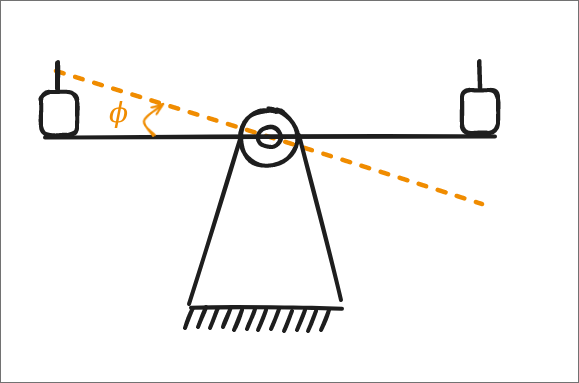
\includegraphics[width=0.6\linewidth]{Figures/schema-simple.png}
	\caption{Schéma Simple du Système}
	\label{fig:system}
\end{figure}

\paragraph{Deux liaisons mécaniques seront utilisées. La première liaison est une liaison pivot qui permet à la barre rotative de tourner autour de l'axe vertical. La deuxième liaison est une liaison encastrement des moteurs à la barre rotative et du support à la base.}

\subsection{Modele 3D}

\paragraph{
	Pour assurer la fixation des moteurs à la barre rotative, on va percer les memes trous existants dans les moteurs dans les deux extrémités de la barre rotative. Ensuite, on va fixer les moteurs à la barre rotative en utilisant des vis.
}
\paragraph*{}
\begin{figure}[!htpb]
	\centering
	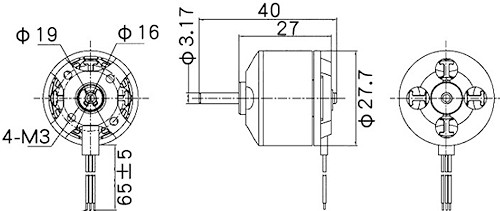
\includegraphics[width=0.6\linewidth]{Figures/motor-draw.jpg}
	\caption{Dessin technique du moteur}
	\label{fig:mobile}
\end{figure}

\paragraph{Pour assurer la fluidité de la rotation de la barre rotative, on va utiliser un roulement à billes pour la liaison pivot. Ce roulement à billes sera fixé à la base et à la barre rotative.}

\paragraph{La partie fixe est composée d'une base qui supporte la barre rotative et une table de bois.}
\begin{figure}[!htpb]
	\centering
	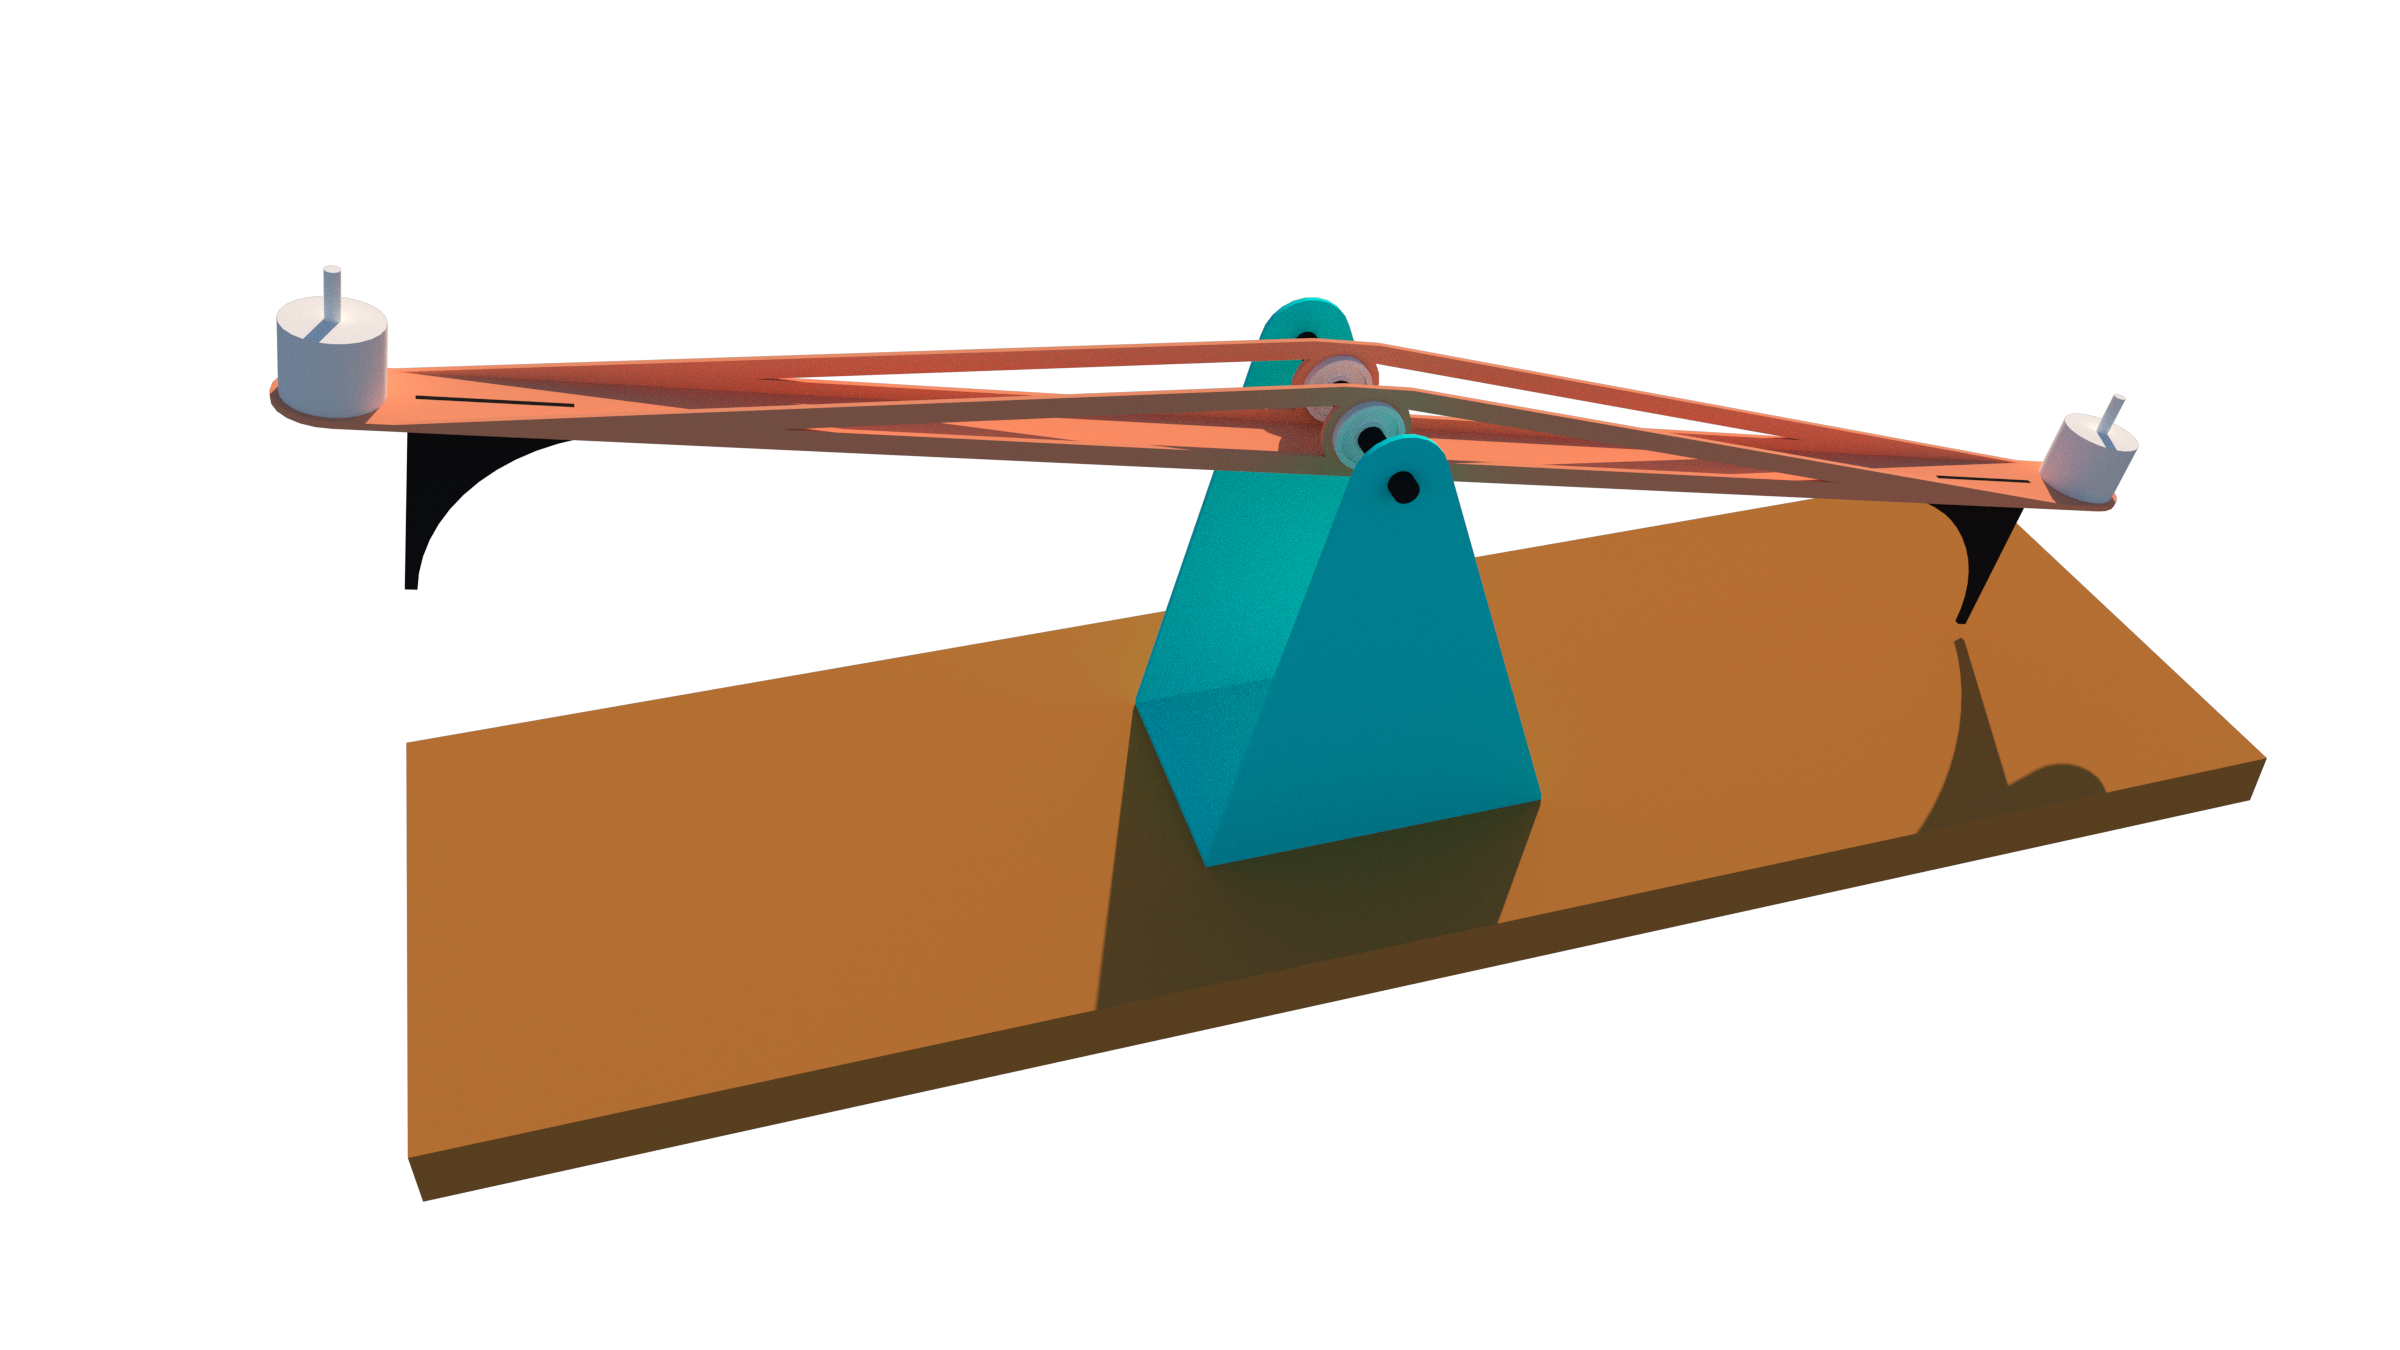
\includegraphics[width=\linewidth]{Figures/3d-cad.png}
	\caption{Modele 3D du design mecanique}
	\label{fig:3d-model}
\end{figure}
\section{Conception Électronique}

\subsection{Carte d'aquisition et de controle}

\paragraph{
	On va utiliser une carte Arduino ATMega 2560 pour la gestion des capteurs et des actionneurs. Cette carte est équipée de plusieurs entrées/sorties numériques et analogiques qui nous permettent de connecter les différents capteurs et actionneurs.
}

\begin{figure}[!htpb]
    \centering
    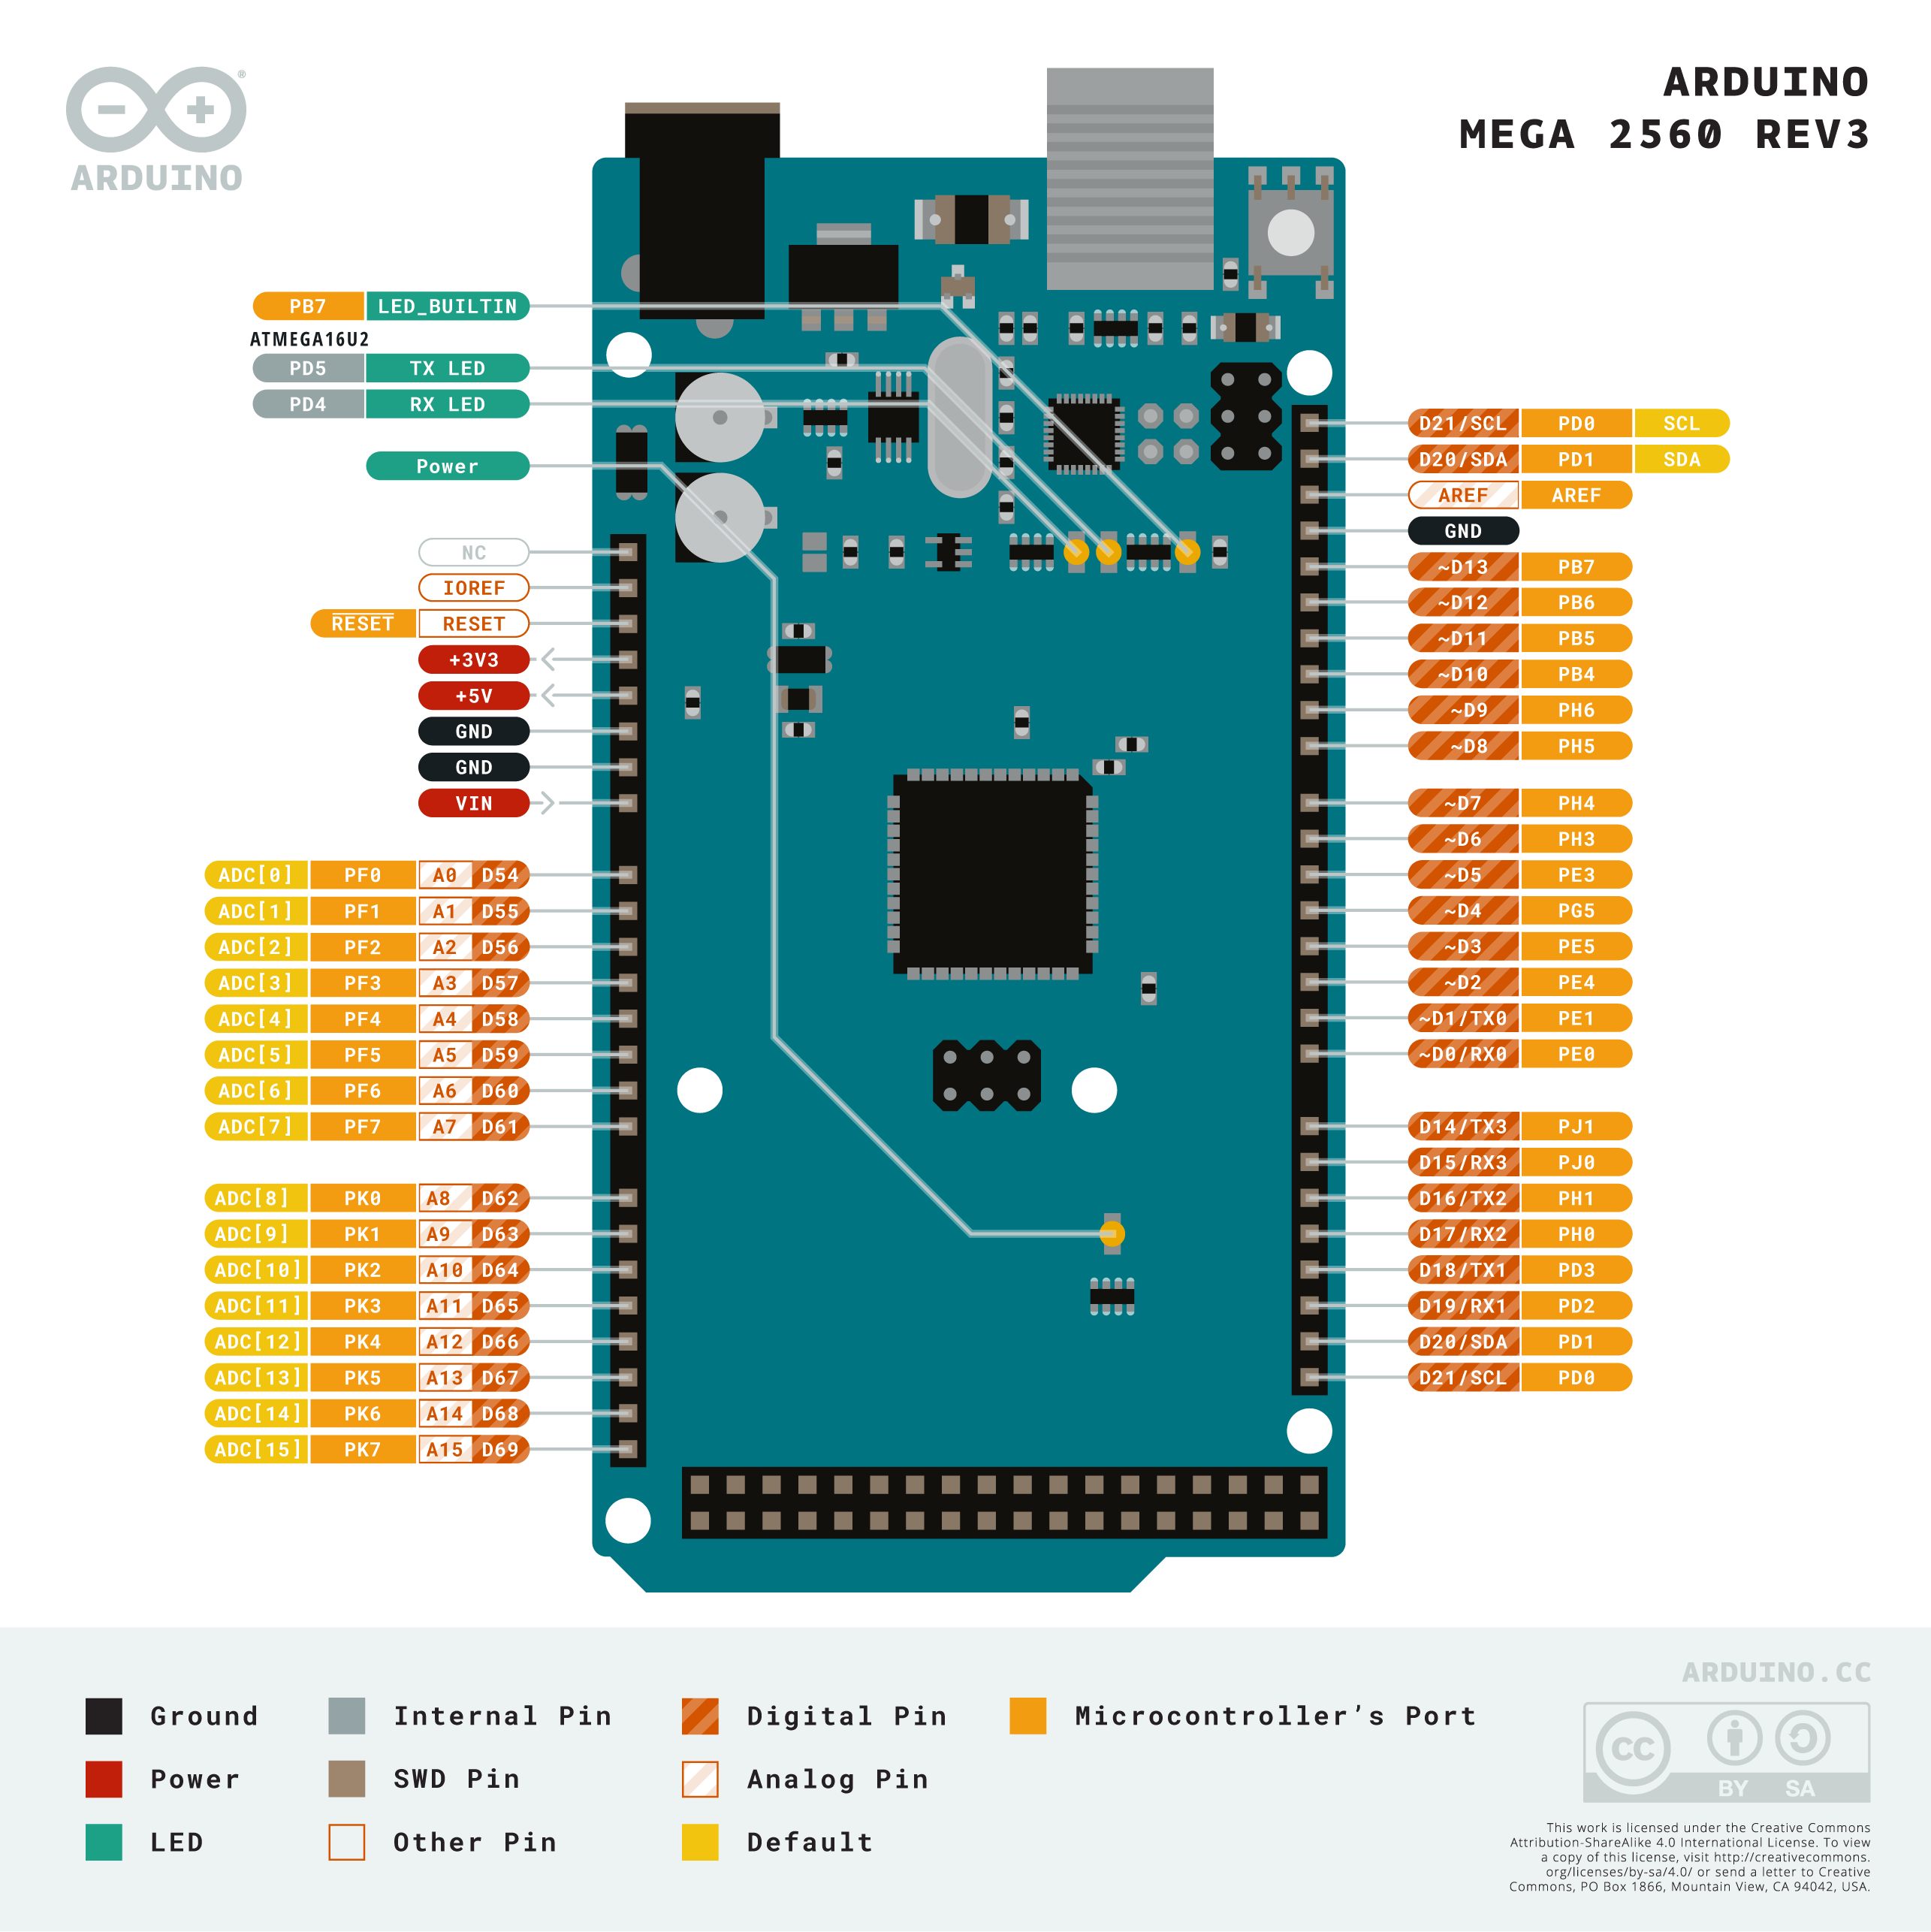
\includegraphics[width=0.6\linewidth]{Figures/arduino.png}
    \caption{Arduino Mega 2560 Pins Layout}
    \label{fig:ArduinoMega2560}
\end{figure}

\paragraph{
	Cette carte peut communiquer en utilisant plusieurs protocoles de communication comme le protocole I2C ou SPI qui nous seront utile pour communiquer avec l'IMU. Aussi, cette carte contient des pins PWM qui nous permettent de contrôler les deux moteurs controlleurs.
}

\subsection{MPU 6050}

\paragraph{Le MPU 6050 est un capteur d'inertie qui combine un accéléromètre et un gyroscope. Il est utilisé pour mesurer l'accélération et la vitesse angulaire. Il communique avec la carte Arduino en utilisant le protocole I2C ou SPI.}

\begin{figure}[!htpb]
	\centering
	\includegraphics[width=0.7\linewidth]{Figures/MPU6050.png}
	\caption{MPU 6050}
	\label{fig:MPU6050}
\end{figure}

\subsubsection{Plages de mesures}

\paragraph{Le MPU 6050 peut mesurer l'accélération selon les trois axes X, Y et Z avec une plage de mesure de $\pm 2g$, $\pm 4g$, $\pm 8g$ et $\pm 16g$. Il peut aussi mesurer la vitesse angulaire selon les trois axes X, Y et Z avec une plage de mesure de $\pm 250$ °$/s$, $\pm 500$ °$/s$, $\pm 1000$ °$/s$ et $\pm 2000$ °$/s$.}

\subsubsection{Pins}

\paragraph{Le MPU 6050 contient 8 pins qui sont :}

\begin{itemize}
	\item VCC : Alimentation 3.3V ou 5V
	\item GND : Masse
	\item SDA : Données I2C
	\item SCL : Horloge I2C
	\item XDA : Données I2C
	\item XCL : Horloge I2C
	\item AD0 : Adresse I2C
	\item INT : Interruption
\end{itemize}

\paragraph{Pour utiliser le MPU on peut utiliser les pins SDA et SCL pour communiquer en utilisant le protocole I2C. Et on laisse AD0 flottant pour utiliser l'adresse x68 par défaut pour l'MPU 6050. Donc on va utiliser les pins SDA, SCL et VCC pour alimenter le MPU 6050 et GND.}

\begin{figure}[!htpb]
	\centering
	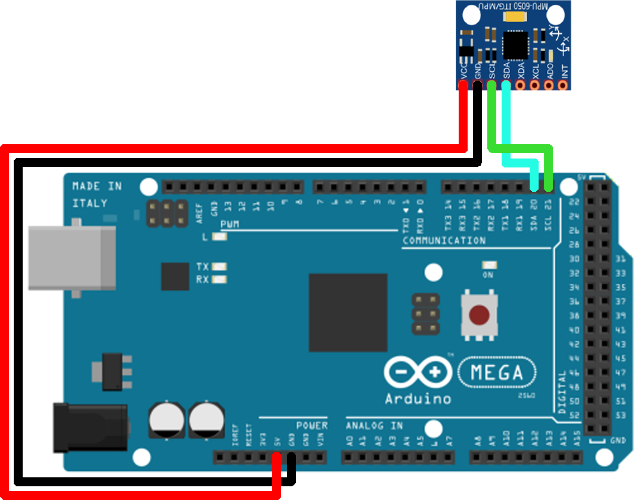
\includegraphics[width=0.7\linewidth]{Figures/mpu-pinning.png}
	\caption{MPU 6050 Pins}
	\label{fig:MPU6050Pins}
\end{figure}

\newpage

\subsection{Moteurs et leurs drivers}

\paragraph{On va utiliser deux moteurs brushless 1000KV pour la propulsion. Ces moteurs sont alimentés et commander par des ESC (Electronic Speed Controller) qui sont des drivers pour les moteurs brushless.}

\paragraph{Ces moteurs contients 3 fils (triphase) qui seront connectés aux ESC.}

\paragraph{Les \gls{esc} sont connectés à la carte Arduino en utilisant les pins PWM pour contrôler la vitesse des moteurs. et alimenter par une batterie LiPo 11.1V.}


\subsubsection{Pinning}

\begin{figure}[!htpb]
	\centering
	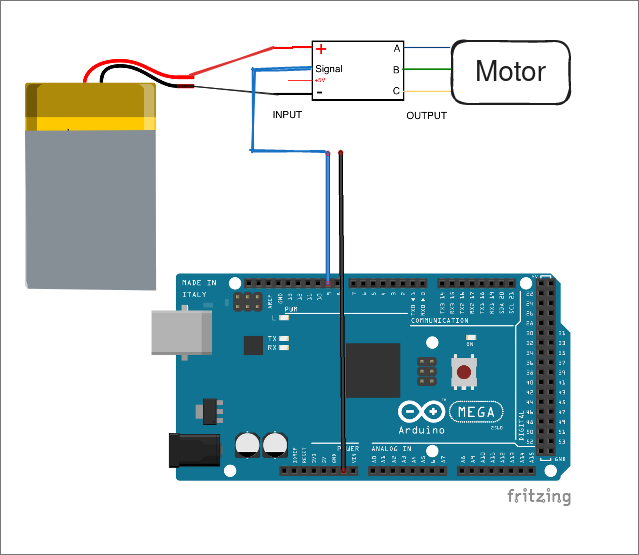
\includegraphics[width=0.5\linewidth]{Figures/esc-motor-pining.png}
	\caption{ESC Pinning}
	\label{fig:ESCPins}
\end{figure}

\subsection{Circuit Electrique}
\paragraph{Apres avoir vu chaque composant du système, nous allons maintenant voir comment les connecter ensemble. La figure \ref{fig:circuit-final} montre le cablage du système.}
\paragraph*{}
\begin{figure}[!htpb]
	\centering
	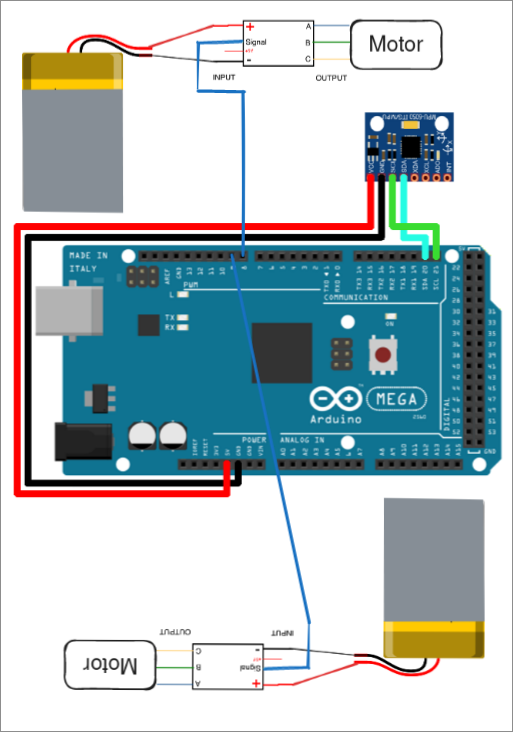
\includegraphics[width=0.9\linewidth]{Figures/final-circuit.png}
	\caption{Circuit Final du Système}
	\label{fig:circuit-final}
\end{figure}

\newpage

\section{Conception du Système de Contrôle}

\paragraph{Dans ce problème, on peut utiliser une commande symetrique pour stabiliser le système. La commande symetrique consiste a utiliser une seule sortie du controlleur PID pour controler les deux moteurs.}

\paragraph{On va utiliser un controlleur PID pour controler la position de la barre rotative. Le controlleur PID va prendre en entrée l'angle de la barre rotative et va donner en sortie la vitesse des moteurs.}


\begin{figure}[!htpb]
	\centering
	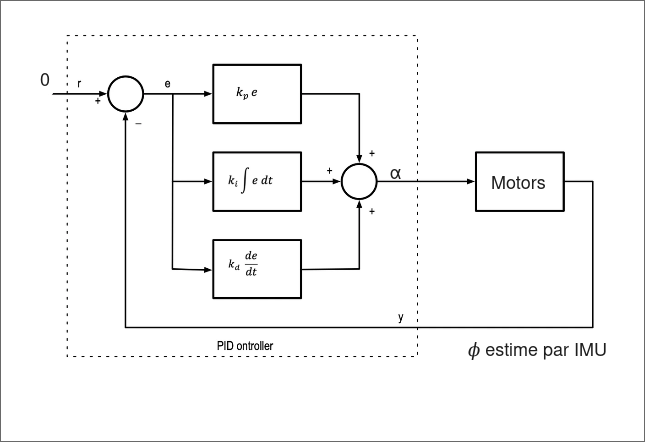
\includegraphics[width=\linewidth]{Figures/pid-schema.png}
	\caption{PID Design}
	\label{fig:pid-design}
\end{figure}

\paragraph{On nomme $\alpha$ la sortie du controlleur PID, $\phi$ l'angle de la barre rotative et $\gamma$ la commande du motor.}
\paragraph{Pour ce systeme on aura une consigne nulle pour stabiliser la barre rotative a $\phi = 0$.}

\paragraph{Donc l'equation du controlleur PID sera :}

\begin{equation}
	\alpha = - K_p \phi - K_i \int \phi dt - K_d \frac{d\phi}{dt}
\end{equation}

\paragraph{Ou $K_p$, $K_i$ et $K_d$ sont les coefficients du controlleur PID.}

\paragraph{Sachant que la commande du moteur est par un signal PWM par $T_{on}$ avec $1000 \leq T_{on} \leq 2000$ (en microsecondes).}

\paragraph{On prends la valeure moyenne centrale de $T_{on}$ et on l'ajoute $\alpha$ pour le premier moteur et on soustrait $\alpha$ pour le deuxieme moteur.}

\paragraph{Donc la commande des moteurs sera :}

\begin{equation}
	\gamma = 1500 \pm \alpha
\end{equation}

\paragraph{Il faut assurer une plage de $\alpha$ adequat pour ne pas depasser la plage de $T_{on}$ des ESC. par exemple $ -400 \leq \alpha \leq 400$. pour ne pas toucher les limites des ESC.}
